\documentclass{article}\usepackage[]{graphicx}\usepackage[]{color}
% maxwidth is the original width if it is less than linewidth
% otherwise use linewidth (to make sure the graphics do not exceed the margin)
\makeatletter
\def\maxwidth{ %
  \ifdim\Gin@nat@width>\linewidth
    \linewidth
  \else
    \Gin@nat@width
  \fi
}
\makeatother

\definecolor{fgcolor}{rgb}{0.345, 0.345, 0.345}
\newcommand{\hlnum}[1]{\textcolor[rgb]{0.686,0.059,0.569}{#1}}%
\newcommand{\hlstr}[1]{\textcolor[rgb]{0.192,0.494,0.8}{#1}}%
\newcommand{\hlcom}[1]{\textcolor[rgb]{0.678,0.584,0.686}{\textit{#1}}}%
\newcommand{\hlopt}[1]{\textcolor[rgb]{0,0,0}{#1}}%
\newcommand{\hlstd}[1]{\textcolor[rgb]{0.345,0.345,0.345}{#1}}%
\newcommand{\hlkwa}[1]{\textcolor[rgb]{0.161,0.373,0.58}{\textbf{#1}}}%
\newcommand{\hlkwb}[1]{\textcolor[rgb]{0.69,0.353,0.396}{#1}}%
\newcommand{\hlkwc}[1]{\textcolor[rgb]{0.333,0.667,0.333}{#1}}%
\newcommand{\hlkwd}[1]{\textcolor[rgb]{0.737,0.353,0.396}{\textbf{#1}}}%
\let\hlipl\hlkwb

\usepackage{framed}
\makeatletter
\newenvironment{kframe}{%
 \def\at@end@of@kframe{}%
 \ifinner\ifhmode%
  \def\at@end@of@kframe{\end{minipage}}%
  \begin{minipage}{\columnwidth}%
 \fi\fi%
 \def\FrameCommand##1{\hskip\@totalleftmargin \hskip-\fboxsep
 \colorbox{shadecolor}{##1}\hskip-\fboxsep
     % There is no \\@totalrightmargin, so:
     \hskip-\linewidth \hskip-\@totalleftmargin \hskip\columnwidth}%
 \MakeFramed {\advance\hsize-\width
   \@totalleftmargin\z@ \linewidth\hsize
   \@setminipage}}%
 {\par\unskip\endMakeFramed%
 \at@end@of@kframe}
\makeatother

\definecolor{shadecolor}{rgb}{.97, .97, .97}
\definecolor{messagecolor}{rgb}{0, 0, 0}
\definecolor{warningcolor}{rgb}{1, 0, 1}
\definecolor{errorcolor}{rgb}{1, 0, 0}
\newenvironment{knitrout}{}{} % an empty environment to be redefined in TeX

\usepackage{alltt}
\usepackage{graphicx}
\usepackage{tabularx}
\usepackage{natbib}

\usepackage{array}
\usepackage{amsmath}
%\usepackage[backend=bibtex]{biblatex}
\bibliographystyle{..//refs/styles/besjournals.bst}
\setkeys{Gin}{width=0.8\textwidth}
%\setlength{\captionmargin}{30pt}
\setlength{\abovecaptionskip}{10pt}
\setlength{\belowcaptionskip}{10pt}
 \topmargin -1.5cm 
 \oddsidemargin -0.04cm 
 \evensidemargin -0.04cm 
 \textwidth 16.59cm
 \textheight 21.94cm 
 \parskip 7.2pt 
\renewcommand{\baselinestretch}{1.2} 	
\parindent 0pt
\renewcommand{\thetable}{S\arabic{table}}
\renewcommand{\thefigure}{S\arabic{figure}}
\usepackage{xr}
\usepackage{xr-hyper}
%\usepackage{hyperref}
\externaldocument{invasive}

\title{Supporting Information: Competition between native Honewort (\textit{Cryptotaenia canadensis}) and invasive Dame's Rocket (\textit{Hesperis matronalis}) seedlings is mediated by relative germination timing}
\IfFileExists{upquote.sty}{\usepackage{upquote}}{}
\begin{document}
\maketitle
\section{Figures}
\begin{figure}[h!]
    \centering
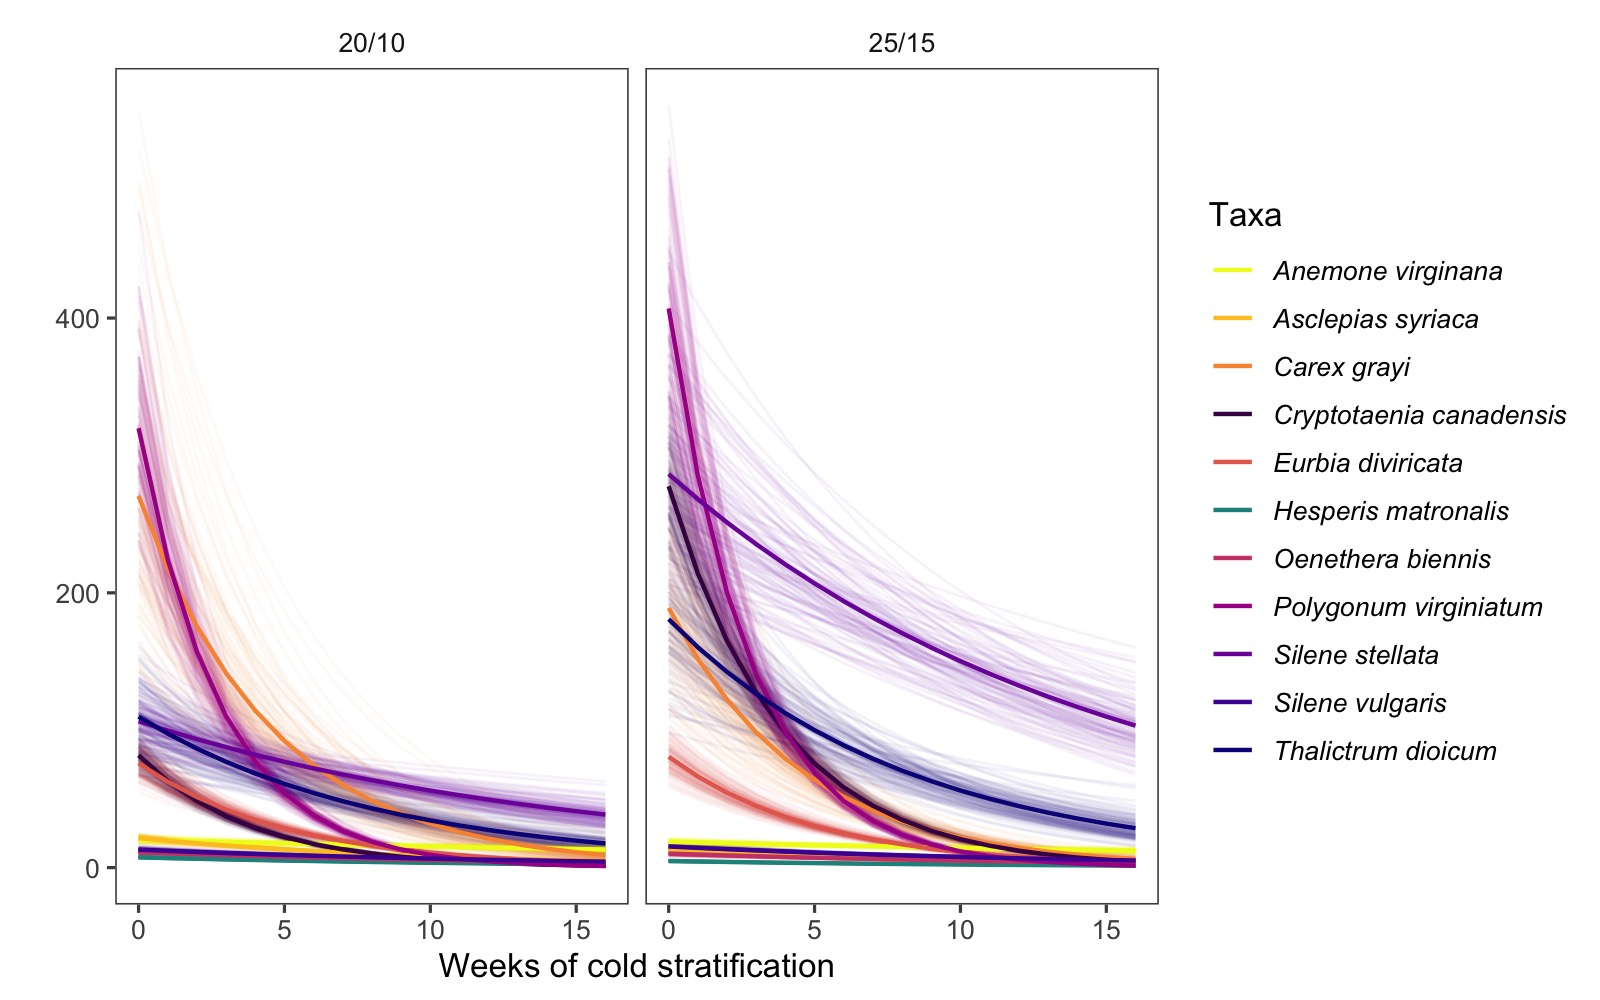
\includegraphics[width=\textwidth]{..//figure/AFTall.jpeg}
   \caption{The effects of weeks of cold stratification at 4\degree C on the time to 50\% germination of 11 herbacious perennials under a) cool and b) warm (20/10\degree C vs. 25/15\degree C day/night) incubation conditions, estimated with accelerated failure time model. The solid lines indicated indicated the mean estimate, while lighter line depict uncertainly with 100 random draws from the posterior distribution.} 
   \label{fig:AFTall}
\end{figure}

\section{Tables}

\begin{table}[ht]
\centering
\begin{tabular}{|rr|ll|ll|}
   \hline
     & & Max germination (\%) & &
   Mean germination time (days) & \\ 
  \hline
  Stratification & Incubation  & C. canadensis & H. matronalis & C. canadensis & H. matronalis \\ 
  \hline
0.00 & H & 0.07 (0.1) & 0.78 (0 & 15.25 (0 & 3.11 (0.6 \\ 
 0.00 & L & 0 (0) & 0.75 (0.1 & --- & 4.59 (0.7 \\ 
   \hline
 2.00 & H & 0.03 (0) & 1 (0 & 9 (1 & 2.3 (0.1 \\ 
 2.00 & L & 0.2 (0.2) & 0.82 (0.1 & 10.25 (0.3 & 2.57 (0.5 \\ 
   \hline
 4.00 & H & 0.18 (0.1) & 0.97 (0 & 9.83 (3.6 & 2.49 (0.3 \\ 
 4.00 & L & 0.58 (0.3) & 0.82 (0.1 & 11.06 (1.1 & 3.5 (0.6 \\ 
    \hline
    5.00 & H & 0.08 (0.1) & 1 (0 & 8.44 (4.7 & 2.33 (0.4 \\ 
 5.00 & L & 0.85 (0.1) & 0.9 (0.1 & 7.67 (0.5 & 2.62 (0.6 \\ 
   \hline
   6.00 & H & 0.25 (0.2) & 0.98 (0 & 13.5 (6.9 & 1.91 (0.2 \\ 
 6.00 & L & 0.77 (0.1) & 0.97 (0.1 & 8.11 (0.4 & 2.14 (0.2 \\ 
    \hline
    7.00 & H & 0.6 (0) & 0.87 (0 & 5.81 (0.2 & 2 (0 \\ 
   7.00 & L & 0.97 (0.1) & 1 (0 & 6.29 (0.2 & 2.15 (0.2 \\ 
    \hline
    8.00 & H & 0.5 (0.1) & 1 (0 & 7.4 (0.3 & 2.06 (0.2 \\ 
   8.00 & L & 0.98 (0) & 0.95 (0 & 6.09 (0.4 & 1.94 (0.1 \\ 
      \hline
   9.00 & H & 0.6 (0.1) & 0.98 (0 & 5.22 (0.7 & 1.74 (0.1 \\ 
   9.00 & L & 1 (0) & 0.93 (0.1 & 6.04 (0.5 & 1.78 (0 \\ 
      \hline
   11.00 & H & 0.73 (0.2) & 0.98 (0 & 4.61 (0.2 & 1.86 (0.1 \\ 
   11.00 & L & 0.93 (0.1) & 0.93 (0.1 & 5.04 (0.3 & 2.11 (0.5 \\ 
      \hline
   13.00 & H & 0.77 (0.2) & 0.88 (0 & 4.14 (0.3 & 1.89 (0.9 \\ 
   13.00 & L & 1 (0) & 0.98 (0 & 4.16 (0.2 & 1.42 (0.3 \\ 
   \hline
\end{tabular}
\caption{Max germination percentages and mean germnation time for our species under all experimental treatment combination. H/L incubation (25 or 20\degree C) and weeks of chilling}
\label{tab:germcomps}
\end{table}




\begin{table}[ht]
\centering
\begin{tabular}{rrrrrrr}
  \hline
 & Estimate & Est.Error & Q2.5 & Q25 & Q75 & Q97.5 \\ 
  \hline
Intercept & 2.59 & 0.25 & 2.10 & 2.41 & 2.76 & 3.09 \\ 
  n\_Cc & -0.41 & 0.03 & -0.47 & -0.43 & -0.38 & -0.34 \\ 
  n\_Hm & 0.12 & 0.03 & 0.07 & 0.11 & 0.14 & 0.17 \\ 
  priority & 0.15 & 0.03 & 0.08 & 0.13 & 0.17 & 0.21 \\ 
   \hline
\end{tabular}
\caption{Estimates from the RGRD models}
\label{tab:RGRD}
\end{table}

\end{document}
